%% jdavid-jdecker-nb-text-classifier.tex
%% Jon David and Jarrett Decker
%% March 2016
%%
%%-------------------------------------------------------------------
%% Notes to self:
%%
%% Package algpseudocode and algorithm need to be installed. Try:
%%   sudo apt-get install texlive-science
%%
%% Adding graphics to LaTeX document:
%%   https://www.sharelatex.com/learn/Inserting_Images


\documentclass{IEEEtran}

\usepackage[style=ieee,backend=bibtex]{biblatex}
\usepackage{hyperref}
\usepackage{amsmath}
\usepackage{algpseudocode}
\usepackage{algorithm}
\usepackage{graphicx}
%%\usepackage{appendix}

%% Tell LaTeX where the images are located
\graphicspath{ {figures/} }

\hypersetup{hidelinks}

%%% ADD RELEVANT REFERENCES HERE %%%
%\addbibresource{quinlan1986.bib}
%\addbibresource{schlimmer1981.bib}
\addbibresource{mitchell1997.bib}



\author{Jarrett Decker*\thanks{e-mail:
    \href{mailto:jdeck069@unm.edu}
         {\texttt{jdeck069@unm.edu}}
         {*authors contributed equally}} and
\and
       Jon David*\thanks{e-mail:
    \href{mailto:jdavid@cs.unm.edu}
         {\texttt{jdavid@cs.unm.edu}}
         {*authors contributed equally}}}

\title{An Implementation of a Naive Bayes Classifier on Text Classification}

\begin{document}

\maketitle

\begin{abstract}

Abstract goes here. Do we really need an abstract?

Keep this example here so we know how to cite references \parencite{mitchell1997machine}.

Keep this here so we know how to do embedded math \LaTeX like $\mathcal{O}(log_{v}n)$
where $v$ is blah blah blah.
\end{abstract}


\section{Introduction}
Naïve Bayes classifiers are a powerful, yet relatively simple, method of doing classification. By leveraging Bayes theorem, the difficult problem of predicting a class based off of a group of attributes can be transformed into the easier task of estimating the chance of those attributes appearing, given a specific class. This is the heart of the Naïve Bayes classification algorithm.

Compared to humans, computers can parse documents incredibly fast, but knowing what the documents are about has traditionally been something only humans can do reliably. With the progress made in machine learning computers can now classify documents at reasonable accuracies. The task of this project was to classify documents into one of twenty “newsgroups” using a Naïve Bayes classifier. Our model did not take word position into account and treated documents as a “bag of words”. 

Naïve Bayes is a good choice for this type of problem because the simplicity of classification allows us to easily handle large data sets, such as all words in the English language.  Naïve Bayes classifiers can also be tweaked through changing beta values in the MAP estimation, or manipulating the data set through things like deleting certain stop words, which could confuse the classifier. This allows you the flexibility to tune your classifier to your problem, making this algorithm useful for many applications, including document classification.

\section{Design and Implementation}
The main features of the Naïve Bayes classifier are the MLE, MAP, and classification functions. Our design modularized these functions through object oriented programming methods, as well as utility functions. 

\section{Data Structures}
Our data necessitated the use of python’s numpy arrays to represent our calculated probabilities. By representing our data in this way, the classification function became a simple addition and matrix multiplication. Along with numpy arrays we also saved our MLE and MAP values to .model files, so we could capture these values and not have to retrain the system every time a classification was run.

\subsection{Naive Bayes Training}
Our design implemented a Trainer class that was in charge of reading in the data and labels and then creating the MLE and MAP models that our classifier uses. This class only has to train once to create the model files and those files are available for classification without having to be retrained. 

The first function of training is to calculate the MLE of the training labels. The purpose of this is to determine the probability of any label appearing for an unknown document. This probability has nothing to do with what words are associated with what labels, just the rate at which labels appear in the training set. {MLE EQUATION AND/OR PSUEDO-CODE FOR MLE FUNCTION}

The second function of training is to determine the MAP of the attributes of the training set. The MAP function allows you to adjust your results to either more resemble what you found in the training set, or to a prior estimation that you can set through the beta value. This beta value is very important, it makes it possible to classify with attributes that you may not have seen for any class before. Usually if you see an attribute that has never been seen belonging to a class, the probability of the unknown class equaling that class will now be zero, but by using the prior beta value instead of zeroing out the probability you can just set it to something small. Since chances are high that classifying combinations of attributes that were not present in the training set, having a beta protects you from having a classification saying there is a zero percent chance of the attributes belonging to any class. {EQUATION/PUESDO-CODE FOR MAP STUFF}

\subsection{Naive Bayes Classification}
We implemented a NaiveBayesClassifier class that was able to use the MLE and MAP from the trainer to do the calculations needed to classify new data. The classifier writes its classifications to a text file in order to be compared to the truth data for the determination of accuracy. 

\subsection{Confuion Matrix and Accuracy}
A confusion matrix is useful for visualizing the results of classification. Accuracy can also be determined from the confusion matrix. We created a ConfusionMatrix class that can read the predicted values that the classifier determined, and the true values from the data set and then increments an element in the confusion matrix associated with those values. For example, if the predicted label was 4 and the true label was 5, the element indexed by [4][5] would be incremented. It follows that elements lying along the diagonal are all accurate predictions while elements off of the diagonal are incorrect. By totaling the values along the diagonal and dividing by the sum of all the values in the matrix the total accuracy of the predictions can be found. 

\subsection{Utility Clases}
To help with the other parts of the program, we added some utility classes. The Vocabulary class was used to store all possible words in our vocabulary and was capable of producing words associated with word IDs and vice versa. The NewsGroups class was similar, except instead of storing information about the words, it stored information about the possible labels, including the size of the set of labels and the names and IDs.

\subsection{Misc. \LaTeX code}
This section contains misc. stuff we might to copy/modify later if we want to use equations, algorithms, and tables.

MAKE SURE THIS SECTION GETS DELETED BEFORE SUBMITTING

\begin{equation}
\label{entropy-equation}
Entropy(S) = \sum_{v\in val(A)}-p_ilog_2(p_i)
\end{equation}


\begin{algorithm}
\caption{calculate information gain($A$, $S$)}
\begin{algorithmic}
\Statex\Comment{ \%Input: attribute A, dataset S\%}
\State $entropybefore$ $\leftarrow$ Entropy($S$)
\State $entropyafter$ $\leftarrow$ 0.0
\For{$v$ $\in$ vals($A$)}
  \State Let $S_v$ $\subseteq$ $S$, such that $S$[$A$] = $v$
  \State $localentropy$ $\leftarrow$ $\frac{|S_v|}{|S|}$ $\times$ Entropy($S_v$)
  \State $entropyafter$ $\leftarrow$ $entropyafter$ + $localentropy$
\EndFor

\State $gain$ $\leftarrow$ $entropybefore$ - $entropyafter$
\State return $gain$
\end{algorithmic}
\end{algorithm}


\section{Experiments}
Talk about the experiments in general...

\subsection{Data}
Talk about the data in detail...

\subsection{Methods}
Talk about the methods in detail...

\subsection{Results}

\begin{figure}
  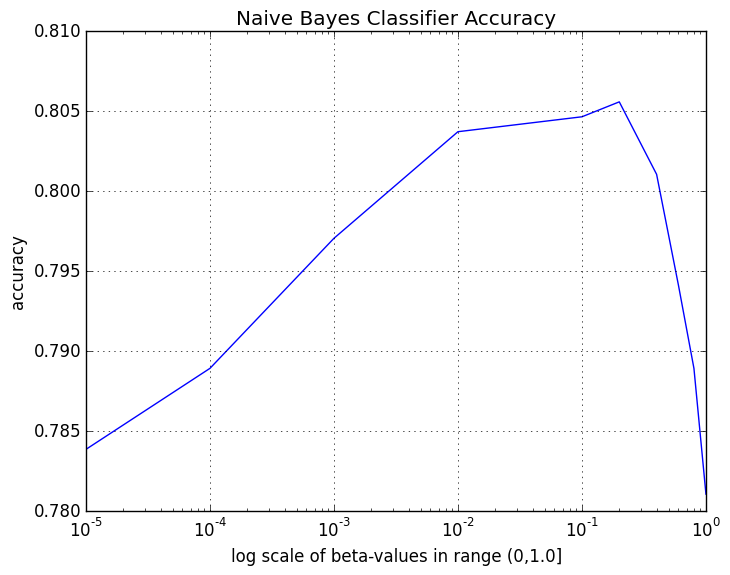
\includegraphics[width=0.5\textwidth, natwidth=80,natheight=80]{betavsacc.png}
  \caption{Performance of classifier with different beta-values}
  \label{fig:betavsacc}
\end{figure}

Figure \ref{fig:betavsacc} shows performance of Naive Bayes Classifier over different values of beta.

Talk about the results in general...

This is how you do a confusion matrix, update it before submitting.
\begin{table}[ht]
  \caption{Confusion Matrix}
  \centering
  \begin{tabular}{c c c }
  \hline\hline
                & Predicted num(p) & Predicted num(e) \\ [0.5ex]
  %heading
  \hline
  Actual num(p) &              985 &                0 \\
  Actual num(e) &                0 &             1048 \\ [1ex]
  \hline
  \end{tabular}
  \label{table:nonlin}
\end{table}

A confusion matrix is more descriptive of a model's performance than
accuracy. A confusion matrix shows the number of true positives (TP), true
negatives (TN), false positives (FP), and false negatives (FN). From this accuracy
and misclassification can be calculated. Accuracy is (TP+TN/p+e) and
Misclassification is 1.0-Accuracy.

In contrast, when evaluating the model over a validation set the label
is not given. The only information provided is accuracy. The table
below shows the classification accuracy of each model over the
validation set.

PUT BETA VS ACCURACY TABLE HERE

\section{Discussion}
Introduce discussion...

\subsection{Comparing Model Options}
Comparison...

\subsection{Explanation of Results}
Explanation...

\subsection{Questions and Answers}
This section answers questions.

%% Question 1
\subsubsection{Explain why it would be difficult to accurately estimate the parameters of this model on a reasonable set of documents.}
The model given is: $(P(Y|X_1 .. X_d) proportional-to P(X_1..d|Y)*P(Y) = P(Y)*PRODUCT(P(X_i|Y)).$
It would be difficult to accurately estimate the parameters of this model on a reasonable set of documents because there are too many (how many?) parameters. For larget data sets estimating the parameters of this model becomes intractable.
Answers go here.

% %% Question 2
% \subsubsection{Report your overall testing accuracy and print out the confusion matrix}
% The accuracy is 80%
% This is what the confusion matrix looks like:

% \begin{table}[ht]
%   \caption{Confusion Matrix}
%   \centering
%   \begin{tabular}{c c c }
%   \hline\hline
%            & 1 & 2 & 3 & 4 & 5 & 6 & 7 & 8 & 9 & 10 & 11 & 12 & 13 & 14 & 15 & 16 & 17 & 18 & 19 & 20\\ [0.5ex]
%   %heading
%   \hline
%   Act.   1 & a & 3 & 4 & 5              985 &                0 \\
%   Act.   1 & a & 3 & 4 & 5              985 &                0 \\
%   Act.   1 & a & 3 & 4 & 5              985 &                0 \\
%   Act.   1 & a & 3 & 4 & 5              985 &                0 \\
%   Act.   1 & a & 3 & 4 & 5              985 &                0 \\
%   Act.   1 & a & 3 & 4 & 5              985 &                0 \\
%   Act.   1 & a & 3 & 4 & 5              985 &                0 \\
%   Act.   1 & a & 3 & 4 & 5              985 &                0 \\
%   Act.   1 & a & 3 & 4 & 5              985 &                0 \\
%   Act.  10 & a & 3 & 4 & 5              985 &                0 \\
%   Act.  11 & a & 3 & 4 & 5              985 &                0 \\
%   Act.  12 & a & 3 & 4 & 5              985 &                0 \\
%   Act.  13 & a & 3 & 4 & 5              985 &                0 \\
%   Act.  14 & a & 3 & 4 & 5              985 &                0 \\
%   Act.  15 & a & 3 & 4 & 5              985 &                0 \\
%   Act.  16 & a & 3 & 4 & 5              985 &                0 \\
%   Act.  17 & a & 3 & 4 & 5              985 &                0 \\
%   Act.  18 & a & 3 & 4 & 5              985 &                0 \\
%   Act.  19 & a & 3 & 4 & 5              985 &                0 \\
%   Act.  20 & a & 3 & 4 & 5              985 &                0 \\
%   \hline
%   \end{tabular}
%   \label{table:nonlin}
% \end{table}


%% Question 3
\subsubsection{Are there any newsgroups that the algorithm confuses more often than others? Why do you think this is?}
asdf

%% Question 4
\subsubsection{Retrain your Naive Bayes classifier for values of beta between 0.00001 and 1 and report the accuracy over the test set for each value of B. Create a plot with values of beta on the x-axis and accuracy on the y-axis. Use a logarithmic scale for the x-axis. Explain in a few sentences why accuracy drops for both small and large values of beta.}
Answers go here.

%% Question 5
\subsubsection{Propose a method for ranking the words in the dataset based on how much the classifier 'relies on' them when performing its classification. It should give high schores to those words that appear frequently in one or a few of the newsgroups but not in other ones. Words that are used frequently in general English should have lower scores, as well as words that only appear extremely rarely throughout the whole dataset.}
Answers go here.

%% Question 6
\subsubsection{Implement your method, set beta back to 1/|V| and print out the 100 words with the highest measure.}
Answers go here.

%% Question 7
\subsubsection{If the points in the training dataset were not sampled independently at random from the same distribution of data we plan to classify in the future, we might call that training set biased. Dataset bias is a problem because the performance of a classifier on a biased dataset will not accurately reflect its future performance in the real world. Look again at the words your classifier is 'relying on'. Do you see any signs of dataset bias?}
Answers go here.

\section{Conclusions}
Hello, conclusions.

\printbibliography

\newpage
\onecolumn
\appendix
\section{Mapping between words and word IDs}
Here are some of the more significant words and their word IDs.

\begin{table}[ht]
  \caption{Selected Word ID and Word mapping}
  \centering
  \begin{tabular}{c c c }
  \hline\hline
                &         Word \\ [0.5ex]
  %heading
  \hline
              1 &            a \\
              2 &           an \\ [1ex]
              3 &          the \\ [1ex]
  \hline
  \end{tabular}
  \label{table:nonlin}
\end{table}



\end{document}